\section{极值与顺序统计量}
\label{sec:rvt-order-statistics}

一台设备由$n$个元件串联而成，任何一个失效设备就停机，寿命是各元件寿命的最小值；若并联，最后一个失效时才停机，寿命是最大值。若关心“第$k$个失效的时刻”，就要把所有寿命排序。这些量都不是光滑的代数运算，但它们的阈值事件很容易写出来。

\paragraph{最大值与最小值}
设$M=\max(X_1,\ldots,X_n)$，$L=\min(X_1,\ldots,X_n)$。最大值不超过$t$，当且仅当每一个都不超过$t$；最小值超过$t$，当且仅当每一个都超过$t$：
\[
 \{M\leq t\}=\bigcap_{i=1}^{n}\{X_i\leq t\},\qquad \{L>t\}=\bigcap_{i=1}^{n}\{X_i>t\} .
\]
所以$F_M(t)$就是联合分布函数在$(t,\ldots,t)$处的值，这一点不需要独立。$X_1,\ldots,X_n$相互独立、分布函数为$F_1,\ldots,F_n$时，交事件的概率分解为乘积：
\begin{equation}
 F_M(t)=\prod_{i=1}^{n}F_i(t),\qquad \mathbb{P}(L>t)=\prod_{i=1}^{n}\bigl(1-F_i(t)\bigr) .
 \label{eq:rvt-max-min}
\end{equation}
没有独立时乘积公式一般不成立。例如$X_2=X_1$时$M=X_1$，$F_M=F_1$，而不是$F_1^2$。

\paragraph{两个例子}
$n$个独立$\operatorname{Unif}(0,1)$的最大值满足$F_M(t)=t^n$，密度$nt^{n-1}$，即$\operatorname{Beta}(n,1)$。$n=2$时$\mathbb{P}(M\leq0.5)=0.25$：图~\ref{fig:rvt-max-min-events}(a)中，$M\leq t$的原像是边长为$t$的小正方形，$L>t$的原像是右上角边长为$1-t$的正方形。

独立的指数寿命$X_i\sim\operatorname{Exp}(\lambda_i)$串联时，由式~\eqref{eq:rvt-max-min}，
\[
 \mathbb{P}(L>t)=\prod_{i=1}^{n}\mathrm{e}^{-\lambda_it}=\mathrm{e}^{-(\lambda_1+\cdots+\lambda_n)t},
\]
所以$L\sim\operatorname{Exp}(\lambda_1+\cdots+\lambda_n)$：失效率相加。取$\lambda=(1,2,3)$，串联寿命服从$\operatorname{Exp}(6)$，均值$1/6$。

还可以问哪个元件最先失效。$X_1$最先失效，即$X_1<\min(X_2,X_3)$；后者服从$\operatorname{Exp}(5)$，且与$X_1$独立。对$X_1$的取值积分，得到
\[
 \mathbb{P}(X_1<\min(X_2,X_3))=\int_0^\infty\mathrm{e}^{-t}\cdot\mathrm{e}^{-5t}\,\mathrm{d}t=\frac16 .
\]
一般地，第$i$个最先失效的概率是$\lambda_i/\sum_j\lambda_j$。

\paragraph{离散情形}
两枚骰子的较大点数$M$，由式~\eqref{eq:rvt-max-min}，$F_M(m)=(m/6)^2$，于是
\begin{equation}
 \mathbb{P}(M=m)=\frac{m^2-(m-1)^2}{36}=\frac{2m-1}{36},\qquad m=1,\ldots,6 .
 \label{eq:rvt-dice-max}
\end{equation}
图~\ref{fig:rvt-max-min-events}(b)中，$M=m$的原像是一个L形，由$m$个横格与$m$个竖格组成，拐角的格子$(m,m)$被两边共用，所以是$2m-1$格而不是$2m$格。这个拐角在后面讨论同值时还会出现。

\begin{BookInlineFigure}
  \centering
  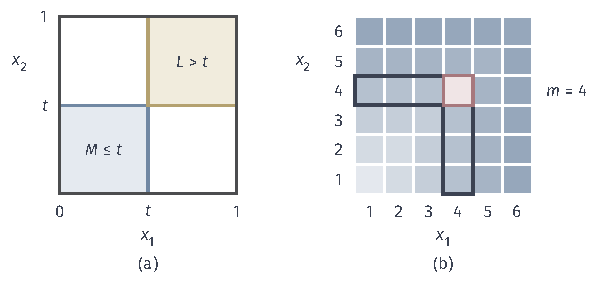
\includegraphics[width=101.3mm]{figures/07-probability/01-elementary-probability/tikz/rvt-max-min-events/figure.pdf}
  \caption{极值事件的原像。(a)单位正方形中，浅蓝正方形是$\max(X_1,X_2)\leq t$，浅黄正方形是$\min(X_1,X_2)>t$，这里$t=0.5$。(b)两枚骰子，同一种蓝色深浅的L形格子较大点数相同，红色格子是$M=m$的L形拐角$(m,m)$，以$m=4$为例共$7$格。}
  \label{fig:rvt-max-min-events}
\end{BookInlineFigure}

\paragraph{顺序统计量}
把$X_1,\ldots,X_n$从小到大排列，记为$X_{(1)}\leq X_{(2)}\leq\cdots\leq X_{(n)}$，$X_{(k)}$称为第$k$个\term{顺序统计量}（order statistic）。$X_{(1)}=L$，$X_{(n)}=M$；$n$为奇数时$X_{((n+1)/2)}$是中间的那个值。

设$X_1,\ldots,X_n$独立同分布，分布函数为$F$。求$X_{(k)}$的分布，关键是把阈值事件改写成计数：$X_{(k)}\leq t$当且仅当至少有$k$个$X_i$不超过$t$。记$N_t$为不超过$t$的个数，它是$n$个示性变量$\mathbf{1}_{\{X_i\leq t\}}$之和。由定理~\ref{thm:rvt-group-independence}，这些示性变量独立，各自以概率$F(t)$取$1$，所以$N_t\sim\operatorname{Bin}(n,F(t))$。

有密度时还可以先看一个直观的计数。$X_{(k)}$落在$[t,t+\Delta t]$，大致意味着：有$k-1$个落在$t$左边，一个落在这一小段里，$n-k$个落在右边。选出这三组的方法有$n!/((k-1)!\,1!\,(n-k)!)$种，每种的概率约为$F(t)^{k-1}\cdot f(t)\Delta t\cdot(1-F(t))^{n-k}$。下面的定理把这个计数严格化。

\begin{theorem}[顺序统计量的分布]
\label{thm:rvt-order-statistics}
设$X_1,\ldots,X_n$独立同分布，分布函数为$F$。
\begin{enumerate}
 \item 对任意$t$与$1\leq k\leq n$，
 \begin{equation}
  \mathbb{P}(X_{(k)}\leq t)=\sum_{j=k}^{n}\binom{n}{j}F(t)^{j}\bigl(1-F(t)\bigr)^{n-j} .
  \label{eq:rvt-order-cdf}
 \end{equation}
 \item 若$F$有密度$f$，则在$f$的连续点处
 \begin{equation}
  f_{X_{(k)}}(t)=\frac{n!}{(k-1)!\,(n-k)!}F(t)^{k-1}\bigl(1-F(t)\bigr)^{n-k}f(t) .
  \label{eq:rvt-order-density}
 \end{equation}
 \item 若$F$有密度$f$，则$(X_{(1)},\ldots,X_{(n)})$有联合密度
 \begin{equation}
  f_{(1),\ldots,(n)}(x_1,\ldots,x_n)=n!\,\prod_{i=1}^{n}f(x_i),\qquad x_1<x_2<\cdots<x_n ,
  \label{eq:rvt-order-joint}
 \end{equation}
 在其他地方为零。
\end{enumerate}
\end{theorem}

\begin{proof}
第一条：$X_{(k)}\leq t$与$N_t\geq k$是同一个事件，而$N_t\sim\operatorname{Bin}(n,F(t))$，把二项质量从$j=k$加到$n$即可。这一步没有用到密度，对含原子的分布同样成立。

第二条：在$f$的连续点处$F'=f$，对式~\eqref{eq:rvt-order-cdf}逐项求导。记$p=F(t)$，第$j$项的导数是
\[
 \binom{n}{j}\Bigl(jp^{j-1}(1-p)^{n-j}-(n-j)p^{j}(1-p)^{n-j-1}\Bigr)f(t) .
\]
利用$\binom{n}{j}j=n\binom{n-1}{j-1}$与$\binom{n}{j}(n-j)=n\binom{n-1}{j}$，并记$a_j=\binom{n-1}{j}p^{j}(1-p)^{n-1-j}$（$a_n=0$），第$j$项化为$nf(t)(a_{j-1}-a_j)$。从$j=k$加到$n$，中间各项相消，只剩
\[
 nf(t)\,a_{k-1}=n\binom{n-1}{k-1}p^{k-1}(1-p)^{n-k}f(t) ,
\]
系数$n\binom{n-1}{k-1}=n!/((k-1)!(n-k)!)$，即式~\eqref{eq:rvt-order-density}。

第三条：排序映射把$\mathbb{R}^{n}$映到$\{x_1<\cdots<x_n\}$。去掉某两个坐标相等的点组成的集合（体积为零）之后，$\mathbb{R}^{n}$按坐标的相对次序分成$n!$个开区域，每个区域上排序映射是一个坐标置换，Jacobian行列式的绝对值为$1$。由式~\eqref{eq:rvt-multivariate-branch}，$n!$个分支各贡献$\prod_if(x_{\pi(i)})$，而乘积与次序无关，都等于$\prod_if(x_i)$，合计$n!\prod_if(x_i)$。
\end{proof}

第三条在$n=2$时就是第~\ref{sec:rvt-branches-reduction}节的排序例子。系数$n!$说明排序把$n!$种次序的质量折叠到同一个有序区域里，这与绝对值变换把两个半轴的质量对折到一起是同一件事。

\paragraph{均匀样本}
$X_i\sim\operatorname{Unif}(0,1)$时$F(t)=t$，$f=1$，式~\eqref{eq:rvt-order-density}成为
\[
 f_{U_{(k)}}(t)=\frac{n!}{(k-1)!\,(n-k)!}t^{k-1}(1-t)^{n-k},\qquad 0<t<1 ,
\]
即$U_{(k)}\sim\operatorname{Beta}(k,n-k+1)$，均值$k/(n+1)$。$n$个点把$[0,1]$分成$n+1$段，由对称性每段的平均长度都是$1/(n+1)$，第$k$个点的平均位置就是$k/(n+1)$。

取$n=3$、$k=2$，三个均匀数的中间值的密度是$6t(1-t)$。由式~\eqref{eq:rvt-order-cdf}，
\[
 \mathbb{P}(U_{(2)}\leq0.25)=3\cdot0.25^2\cdot0.75+0.25^3=0.140625+0.015625=0.15625 .
\]
对密度积分也得到同一个值：
\[
 \int_0^{0.25}6t(1-t)\,\mathrm{d}t=3\cdot0.25^2-2\cdot0.25^3=0.15625 .
\]图~\ref{fig:rvt-order-stats}画出$n=5$时五个顺序统计量的密度。

\begin{BookInlineFigure}
  \centering
  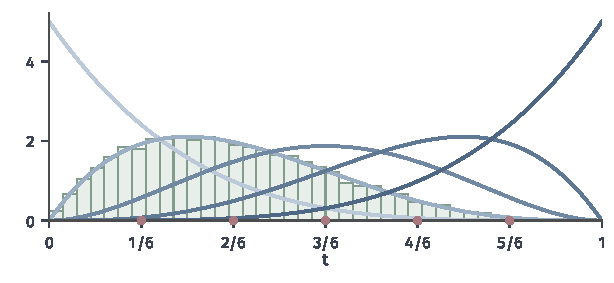
\includegraphics[width=104mm]{figures/07-probability/01-elementary-probability/matplotlib/rvt-order-stats/figure.pdf}
  \caption{$n=5$个独立$\operatorname{Unif}(0,1)$的顺序统计量。蓝色由浅到深是$U_{(1)},\ldots,U_{(5)}$的密度$\operatorname{Beta}(k,6-k)$，红点标出均值$k/6$；浅绿直方图是$20000$组模拟样本中$U_{(2)}$的值（种子$19$）。}
  \label{fig:rvt-order-stats}
\end{BookInlineFigure}

\paragraph{同值与原子}
式~\eqref{eq:rvt-order-density}与式~\eqref{eq:rvt-order-joint}依赖一件事：样本两两不同的概率为$1$，这样$n!$种次序互不重叠。分布有原子时，同值出现的概率为正，两枚骰子点数相同的概率就是$1/6$，这时按$n!$个分支计数会重复计算。

骰子的最大值说明了这一点。若仿照式~\eqref{eq:rvt-order-density}，用$2F(m)p(m)$代替$\mathbb{P}(M=m)$，得到$2m/36$，对$m$求和是
\[
 \sum_{m=1}^{6}\frac{2m}{36}=\frac{42}{36}>1 .
\]
多出的$6/36$恰好是六个对角格子$(m,m)$：它们在“第一枚最大”与“第二枚最大”两个分支中各被算了一次。正确的计数是式~\eqref{eq:rvt-dice-max}的$2m-1$。

有原子时应回到式~\eqref{eq:rvt-order-cdf}，它只用了计数$N_t$，对任何分布都成立。离散变量的质量由分布函数的跳跃得到：记$F(t^-)=\mathbb{P}(X<t)$，把式~\eqref{eq:rvt-order-cdf}中的$F(t)$换成$F(t^-)$就得到$\mathbb{P}(X_{(k)}<t)$，两者相减就是$\mathbb{P}(X_{(k)}=t)$。

以三枚骰子的中间点数为例，求它等于$3$的概率。$F(3)=1/2$，$F(3^-)=F(2)=1/3$，代入式~\eqref{eq:rvt-order-cdf}，
\[
 \mathbb{P}(X_{(2)}\leq3)=3\cdot\frac14\cdot\frac12+\frac18=\frac12,\qquad \mathbb{P}(X_{(2)}<3)=3\cdot\frac19\cdot\frac23+\frac1{27}=\frac{7}{27} .
\]
两者之差是$\mathbb{P}(X_{(2)}=3)=1/2-7/27=13/54\approx0.241$，直接枚举$216$种结果也得到$52$种，即$52/216=13/54$。
